

\documentclass[a4paper]{article} 
\addtolength{\hoffset}{-2.25cm}
\addtolength{\textwidth}{4.5cm}
\addtolength{\voffset}{-3.25cm}
\addtolength{\textheight}{5cm}
\setlength{\parskip}{0pt}
\setlength{\parindent}{0in}

%----------------------------------------------------------------------------------------
%	PACKAGES AND OTHER DOCUMENT CONFIGURATIONS
%----------------------------------------------------------------------------------------

\usepackage{blindtext} % Package to generate dummy text
\usepackage{charter} % Use the Charter font
\usepackage[utf8]{inputenc} % Use UTF-8 encoding
\usepackage{microtype} % Slightly tweak font spacing for aesthetics
\usepackage[english, spanish, es-nodecimaldot]{babel} % Language hyphenation and typographical rules
\usepackage{amsthm, amsmath, amssymb} % Mathematical typesetting
\usepackage{float} % Improved interface for floating objects
\usepackage[final, colorlinks = true, 
            linkcolor = black, 
            citecolor = black]{hyperref} % For hyperlinks in the PDF
\usepackage{graphicx, multicol} % Enhanced support for graphics
\usepackage{xcolor} % Driver-independent color extensions
\usepackage{marvosym, wasysym} % More symbols
\usepackage{rotating} % Rotation tools
\usepackage{censor} % Facilities for controlling restricted text
\usepackage{listings, style/lstlisting} % Environment for non-formatted code, !uses style file!
\usepackage{pseudocode} % Environment for specifying algorithms in a natural way
\usepackage{style/avm} % Environment for f-structures, !uses style file!
\usepackage{booktabs} % Enhances quality of tables
\usepackage{tikz-qtree} % Easy tree drawing tool
\usepackage{enumitem}  
\usepackage{graphicx} 
\usepackage{booktabs}
\usepackage{array}  
\usepackage{bm}
\tikzset{every tree node/.style={align=center,anchor=north},
         level distance=2cm} % Configuration for q-trees
\usepackage{style/btree} % Configuration for b-trees and b+-trees, !uses style file!
\usepackage[backend=biber,style=numeric,
            sorting=nyt]{biblatex} % Complete reimplementation of bibliographic facilities
\addbibresource{sample.bib}
\usepackage{csquotes} % Context sensitive quotation facilities
\usepackage[yyyymmdd]{datetime} % Uses YEAR-MONTH-DAY format for dates
\renewcommand{\dateseparator}{-} % Sets dateseparator to '-'
\usepackage{fancyhdr} % Headers and footers
\pagestyle{fancy} % All pages have headers and footers
\fancyhead{}\renewcommand{\headrulewidth}{0pt} % Blank out the default header
\fancyfoot[L]{} % Custom footer text
\fancyfoot[C]{} % Custom footer text
\fancyfoot[R]{\thepage} % Custom footer text
\newcommand{\note}[1]{\marginpar{\scriptsize \textcolor{red}{#1}}} % Enables comments in red on margin
\DeclareMathOperator*{\plim}{plim}
\usepackage[most]{tcolorbox}
\usepackage{cancel}
\usepackage{adjustbox}
\addto\captionsspanish{
\def\listtablename{\'Indice de tablas}%
\def\tablename{Tabla}}
\usepackage{xcolor}
\usepackage{multirow}
\usepackage{listings}
\usepackage{bbm}
\newcommand{\indep}{\perp\!\!\!\!\perp} 
\definecolor{myblue}{RGB}{0,163,243}
\definecolor{moradito}{RGB}{63,1,143}

\usepackage{tcolorbox}
\newtcolorbox{solucion}{colbacktitle=gray, coltitle=white, breakable,
colframe=black, colback=white, fonttitle=\bfseries,parbox=true,
title=Solución:}
\usepackage{float}

\usepackage{listings,xcolor}
\usepackage{upquote}
 
\usepackage[spanish]{babel}
\usepackage{enumerate}
\usepackage{hyperref} 
%\decimalpoint
\setlength\parindent{0pt}
\newcommand*{\QED}{\hfill\ensuremath{\blacksquare}}
\usepackage{authblk}
\selectlanguage{spanish}

\newtheorem{theorem}{Teorema}[section]
\newtheorem{corollary}{Corolario}[theorem]
\newtheorem{lemma}[theorem]{Lema}
\theoremstyle{remark}
\newtheorem*{remark}{Considere}
\DeclareUnicodeCharacter{2212}{-}
\usepackage{epigraph}

%\usepackage[natbibapa]{apacite}
\usepackage{tikz}
\usepackage{physics}
\newcommand{\ubar}[1]{\text{\b{$#1$}}}

\usepackage{tcolorbox}


\usepackage{float}

\usepackage{listings,xcolor}
\usepackage{upquote}
\usepackage{subfigure}

 
\theoremstyle{definition}
\newtheorem{definition}{Definición}[section]

\usepackage{listings}
\usepackage{xcolor}

% Configuración para resaltar código MATLAB
\lstset{
    language=Matlab, % Indica el lenguaje para resaltar
    basicstyle=\ttfamily\small, % Estilo básico del texto
    keywordstyle=\color{blue}, % Estilo para palabras clave
    commentstyle=\color{green}, % Estilo para comentarios
    stringstyle=\color{red}, % Estilo para cadenas de texto
    numberstyle=\tiny\color{gray}, % Estilo para números de línea
    stepnumber=1, % Incremento entre números de línea
    numbersep=10pt, % Espacio entre números y código
    backgroundcolor=\color{white}, % Color de fondo del código
    showstringspaces=false, % Evitar espacios para cadenas de texto
    breaklines=true, % Permitir líneas largas se corten
    frame=single, % Crear un borde alrededor del bloque de código
}


%Código para imágenes
%\begin{figure}[H]
%\centering
%\includegraphics[scale=0.5]{PIB.png}
%\caption{Crecimiento porcentual del PIB desde 1990 hasta 2009}
%\end{figure}

\usepackage{amsmath}
\usepackage[utf8]{inputenc}
\usepackage[spanish]{babel}
\usepackage{amsmath}
\usepackage{amsfonts}
\usepackage{amssymb}
\usepackage{hyperref}
\title{Big Data y Machine Learning: Problem Set 2}
\author{Ignacio Sarmiento}

\date{20 de Octubre de 2024}

\begin{document}
\maketitle

\begin{center}

\begin{tabular}{ c c c }
 \textbf{Integrantes:} & Juliet Alejandra Molano Rizo & 202226070 \\
 & Henry Nicolas Carvajal Cardenas & 201718787\\
 & Diego Fernando Cuesta Mora & 202315672\\
 & Jorge Ramirez Sanchez & 202116747
\end{tabular}

\end{center}

%-------------------------------------------------%
\section{Introducción} \\

La pobreza monetaria extrema sigue siendo uno de los principales retos globales, afectando aproximadamente al 9,2\% de la población mundial o alrededor de 700 millones de personas, según el Banco Mundial (2023). La mayoría de los afectados se encuentra en áreas de África Subsahariana y Asia Meridional, donde la falta de acceso a servicios básicos y oportunidades económicas limita significativamente el desarrollo. En América Latina, los avances en reducción de la pobreza extrema se ven amenazados tras la pandemia de COVID-19, que ha aumentado el número de personas en situación de pobreza. En Colombia, la situación es especialmente preocupante, con cerca de 33,0\% de la población en pobreza monetaria y 11,4\% en pobreza monetaria extrema, cifras que alcanzan niveles más altos en zonas rurales (DANE, 2023). \\

La pobreza tiene implicaciones profundas en la salud, educación y oportunidades, perpetuando ciclos de desigualdad y limitando el progreso económico de los países. Los altos niveles de pobreza restringen la capacidad de las naciones para avanzar en términos de bienestar general y competitividad económica. Esta situación exige el desarrollo de enfoques que permitan identificar y priorizar intervenciones de política eficaces para reducir la pobreza. En este contexto, la predicción de la pobreza resulta clave, ya que facilita la toma de decisiones en políticas públicas y permite focalizar los recursos en los hogares más vulnerables. Las técnicas de big data y machine learning proporcionan herramientas avanzadas para realizar predicciones más precisas, lo que contribuye a mejorar la eficiencia y efectividad de las políticas destinadas a combatir la pobreza (Sosa \& Cornejo, 2022).\\ 

La predicción de la pobreza en América Latina ha evolucionado con metodologías que integran enfoques de aprendizaje automático y datos combinados. Un ejemplo destacado es el estudio de Sosa y Cornejo (2022) para la CEPAL, que emplea un enfoque “micro-macro” para predecir la tasa de pobreza en varios países de la región. Esta metodología combina datos macroeconómicos agregados con encuestas de hogares a nivel micro, incluyendo variables como microdatos de ingresos, tasa de variación del ingreso medio y del coeficiente de Gini para cada país y período. Al comparar los resultados de 2019, este modelo base logró un desempeño notable, obteniendo un puntaje F1 de hasta 0.878 para Honduras, mientras que otros países lograron puntuaciones entre 0.3 y 0.7. Esta metodología también explora modelos de aprendizaje automático, evaluando su efectividad en la predicción de grupos específicos, como mujeres y jóvenes, para maximizar la precisión y relevancia de las políticas públicas en la región. \\

Otros estudios complementan esta visión, como el trabajo de Muñetón-Santa y Manrique-Ruiz (2023) que emplea datos espaciales a nivel de manzana para estimar el índice de pobreza multidimensional en Medellín, Colombia. Utilizando algoritmos como XGBoost, LightGBM y Random Forest, encontraron que el modelo lineal general (GLM) y Random Forest eran los más eficaces, con un MAE de 0.075 para este último. Esto refuerza la aplicabilidad de datos geoespaciales en la evaluación de la pobreza y la alta correlación entre la distribución espacial y los niveles reales de pobreza en la región. Otro trabajo en esta línea es el análisis de Sabogal, García-Bedoya y Granados (2021) en Colombia, donde el algoritmo XGBoost  mostró un rendimiento F1 de 0.96, destacando variables predictivas claves como educación, empleo, salud y características de las viviendas, lo cual resulta esencial para una evaluación precisa de la pobreza y la vulnerabilidad estructural. \\

%---------------------------------------------------------------


Medir y predecir la pobreza es fundamental para identificar los hogares más vulnerables y comprender los factores que contribuyen a su situación. Una medición precisa permite a los gobiernos ajustar sus políticas y garantizar que los recursos se destinen de manera eficiente. Los modelos predictivos juegan un papel clave al mejorar la identificación de hogares en riesgo, facilitando una respuesta más ágil y efectiva, especialmente en situaciones de crisis. Esta capacidad de anticipación no solo optimiza los esfuerzos de reducción de la pobreza, sino que también contribuye a mitigar riesgos y promover una sociedad más equitativa.\\

Desde finales de los años 80, Colombia ha adoptado diferentes metodologías para medir la pobreza, destacándose la medición de la pobreza monetaria calculada por el DANE. Esta medida evalúa la capacidad de un hogar para adquirir una canasta básica de alimentos y bienes esenciales, con un umbral que, en 2018, se fijó en \$275.594 pesos mensuales. En este estudio se utiliza esta medida para llevar a cabo un análisis predictivo de la pobreza, empleando datos del DANE y la misión “Empalme de las Series de Empleo, Pobreza y Desigualdad - MESE”, que abarcan tanto ingresos del hogar como otras dimensiones socioeconómicas y características de sus miembros. Específicamente, los datos contienen cuatro conjuntos divididos en ‘entrenamiento’ y ‘prueba’ a nivel hogar e individual.\\

El estudio se enfoca en desarrollar un modelo predictivo de la pobreza en Colombia, basado en estos datos. El modelo, diseñado a nivel de hogar, busca maximizar la eficiencia utilizando un conjunto mínimo de variables, lo que reduce los costos de las encuestas tradicionales. A diferencia de enfoques anteriores, este modelo abordará la pobreza como un problema de clasificación, categorizando a los hogares como pobres o no pobres en función de sus características socioeconómicas y demográficas, tanto del hogar como de sus miembros. Esta metodología permitirá comprender mejor la distribución de la pobreza e identificar los factores más determinantes en la vulnerabilidad económica de los hogares, facilitando la creación de políticas públicas más focalizadas y efectivas. \\

El modelo de clasificación más eficiente se alcanzó empleando el algoritmo XGboost , el cual logra clasificar con gran precisión a los hogares como pobres o no pobres, utilizando características socioeconómicas y demográficas clave, como la afiliación a la seguridad social de los miembros del hogar, el nivel de educación máximo alcanzado por algún miembro del hogar, el número de ocupados, entre otras. En la base de entrenamiento, el modelo alcanzó una puntuación F1 de 0.90\%, mientras que en la plataforma Kaggle se obtuvo una puntuación de 0.683\%, demostrando su robustez y capacidad para generalizar con datos fuera de muestra.\\

Con el objetivo de que los resultados sean replicables, el trabajo cuenta con un \href{https://github.com/HenryC2/Problem-Set-2_Machine-Learning_2024.git}{repositorio en GitHub}. El repositorio cuenta con cuatro carpetas. La carpeta 'Base' contiene las bases de datos utilizadas en el ejercicio, contemplando tanto las bases originales como las rebalanceadas a través de la metodología SMOTE. La segunda carpeta denominada 'Códigos' contiene el conjunto de programas R con los que se intentó, a través de diferentes metodologías, predecir la pobreza. La tercera carpeta denominada 'Gráficas' contiene las gráficas que se utilizaron en el análisis de los datos. La cuarta carpeta denominada 'Output' almacena los resultados del proceso de clasificación de la pobreza que se subieron a la plataforma Kaggle. 


\section{Datos}

\textbf{2.1 Descripción de los datos} \\


El set de datos original, del cual se origina la muestra utilizada en este taller, provienen de la Misión de Empalme de las Series de Empleo, Pobreza y Desigualdad (MESE) del DANE. Este ejercicio fue creado en 2009 a través de un convenio entre el DANE y el DNP, el cual se encargó de evaluar y comparar la información entre la Encuesta Continua de Hogares (ECH) y la Gran Encuesta Integrada de Hogares (GEIH). \\

El objetivo de estos datos es evaluar la pobreza de los hogares utilizando tanto el método directo como el indirecto, lo que permite una metodología más precisa para medir la pobreza en Colombia, tanto a nivel individual como de hogar. De esta forma, los datos consideran los hábitos y capacidades disponibles de la población. La muestra incluye variables que permiten evaluar la satisfacción de necesidades básicas en los hogares, la distribución de ingresos a lo largo del tiempo mediante el empalme entre encuestas, y características relacionadas con la vivienda y los miembros del hogar. \\

Tomando esto en cuenta, se analizó el conjunto de datos del ejercicio. La base de entrenamiento para hogares contiene 23 variables y 164.960 registros, mientras que la base de personas incluye 135 variables y 543,109 registros. Por su parte, las bases de testeo cuentan con 16 variables y 66,168 observaciones para hogares, y 63 variables y 219,644 observaciones para personas. Se realizó un análisis de valores faltantes para identificar las variables con datos incompletos. Además, dado que el objetivo del ejercicio se enfoca en los hogares, se agruparon las principales variables de interés, considerando el identificador del hogar y la persona que actúa como jefe del mismo.\\

El desafío de la predicción radica en que las bases de testeo no incluyen información sobre el ingreso del hogar. El objetivo de la predicción es determinar si un hogar es pobre o no, utilizando las variables disponibles a nivel hogar y creando algunas nuevas variables a partir de la base de personas. Esto es posible porque ambas bases comparten una variable común, 'id', que identifica el hogar al que pertenece cada persona. Otro aspecto importante a tener en cuenta es la posible correlación entre las variables relacionadas con el tamaño del hogar, ya que variables como el número de habitaciones o el número de miembros pueden estar correlacionadas, lo que podría distorsionar los resultados del modelo.\\

Igualmente, para lograr una correcta evaluación de la pobreza, como menciona Atkinson(1987), implica considerar múltiples variables más allá del ingreso. Estas incluyen el tamaño y la composición del hogar, las necesidades específicas como salud o edad, el acceso a servicios básicos como educación y vivienda, entre otros aspectos. Además, las condiciones de vida, el nivel educativo, la estabilidad laboral y las redes de apoyo social también influyen significativamente en la capacidad de una persona para superar la pobreza, mostrando que la pobreza es un fenómeno multidimensional.\\

En general, las variables seleccionadas están diseñadas para describir los factores que influyen en la pobreza de los hogares, tales como el número de niños, nivel educativo, cantidad de habitaciones por persona y ubicación geográfica, entre otros. También se utilizan variables relacionadas con las características socioeconómicas del jefe de hogar, como la edad, la educación, fuentes de ingresos y la situación laboral, para capturar mejor la realidad económica de cada hogar.\\

\textbf{2.2 Limpieza de datos y selección de variables} \\

En esta sección se explicará el procedimiento llevado a cabo para el tratamiento de las bases de datos con respecto a personas y hogares, tanto en las fases de entrenamiento (train) como de prueba (test). Se detallará el proceso realizado para transformar las bases de datos de personas en bases con respecto al hogar, la selección de variables relevantes, y finalmente, la integración de todas las bases. A continuación, se describirá paso a paso el procedimiento aplicado.\\

\begin{itemize}
    \item \textbf{
Procesamiento de la base de datos de personas para su conversión a nivel de hogar en las bases de entrenamiento (Train) y prueba (Test)} \\


Como primer paso, se seleccionaron las variables compartidas entre las bases de datos de entrenamiento y prueba a nivel de personas. Luego, se crearon variables dummies para aquellas variables que preliminarmente se consideraron de interés. Para las variables categóricas con valores faltantes, como el nivel educativo, se asignó el menor nivel educativo del hogar, dado que las personas comparten el identificador del hogar. En otras variables con valores perdidos (NAs), estos se reemplazaron por cero.\\

Es importante destacar que, para crear una base de datos a nivel de personas, se generaron inicialmente dos sub-bases para luego combinarlas. La primera sub-base agrupó la información a nivel del hogar, incluyendo el número de niños (menores de 6 años), el número de adultos (mayores de 30 años), el número de desempleados, inactivos, incapacitados, y el número de personas que reciben subsidios del gobierno, entre otros. La segunda sub-base contenía información a nivel del jefe de hogar, considerando variables como si el jefe es mujer, datos socioeconómicos como nivel educativo, edad, afiliación al régimen subsidiado, contribución a pensión, ingresos, situación laboral, entre otros. Ambas sub-bases se unieron a través del identificador del hogar ("id") para obtener una base completa a nivel de hogar.\\



    \item \textbf{Procesamiento de la base de datos a nivel de hogar en las bases de entrenamiento (Train) y prueba (Test)} \\

En este proceso de tratamiento de datos, se renombraron varias variables en las bases de datos de hogares para mejorar su interpretación. Por ejemplo, se renombraron las variables correspondientes al número total de cuartos disponibles en el hogar, los cuartos donde duermen las personas, el tipo de vivienda, y los pagos mensuales de amortización o arriendo. Además, se crearon nuevas variables, como el número de personas por cuarto donde duermen y una variable de hacinamiento, que indica si más de tres personas comparten el mismo cuarto. Este tratamiento se aplicó tanto a la base de entrenamiento como a la de prueba para asegurar la consistencia de los datos. \\

Por último, se integraron las bases de datos de personas con las de hogares, tanto para los conjuntos de entrenamiento como para los de testeo, utilizando el identificador único de cada hogar. A continuación, se aplicó una función para modificar y decodificar varias variables. Se transformaron en factores las variables relacionadas con el dominio, oficio, ocupación del jefe de hogar, tipo de vivienda, nivel educativo del jefe de hogar y el nivel educativo máximo en el hogar, entre otras. Además, se creó la variable “Cabecera” para identificar si el hogar estaba ubicado en una zona urbana, y los valores faltantes se ajustaron convirtiéndolos en ceros. Finalmente, dada la importancia de la variable de valor del arriendo del hogar en la predicción de la pobreza, una vez que puede limitar el ingreso disponible del hogar, se imputó información a los datos faltantes utilizando la pregunta de la encuesta: Si tuviera que pagar arriendo por esta vivienda,¿cuánto estima que tendría que pagar mensualmente? \\

    \item \textbf{Rebalanceo de la base de datos mediante SMOTE.} \\

Es importante notar que la base de datos presenta un problema de desbalance en la variable objetivo. Este desbalance surge porque solo el 20.01\% de los hogares en la base de entrenamiento son clasificados como pobres, mientras que el 79.99\% restante no lo son. Este desbalance es un problema porque los modelos de machine learning tienden a enfocarse en predecir la clase mayoritaria, lo que daría como resultado un modelo que predice con alta precisión los hogares no pobres, pero con baja capacidad para identificar los hogares pobres, que es el objetivo principal. En este caso generamos observaciones sintéticas hacia arriba para la clase pobre.\\

Para abordar este problema, utilizamos SMOTE (Synthetic Minority Over-sampling Technique). Generamos nuevas observaciones sintéticas de la clase minoritaria (en este caso, los hogares pobres) mediante la creación de ejemplos intermedios entre las observaciones reales existentes. Esto permite balancear la distribución de las clases en la base de datos, mejorando la capacidad del modelo para aprender y predecir correctamente tanto la clase mayoritaria como la minoritaria, lo que en este caso es crucial para predecir con precisión la pobreza. En este caso decidimos probar 2 opciones, aproximar 5 y a 10 observaciones cercanas para generar las observaciones sintéticas.
    
\end{itemize}

Por último, para abordar diferentes sets de variable y pruebas entre la base original y los datos procesados, se realizó un proceso de estimación, probando diferentes conjuntos de variables y observando su capacidad de predecir por fuera de la muestra de entrenamiento a través del F1-Score. Al ser esta una métrica que combina la precisión y la sensibilidad, permitió evaluar el equilibrio entre falsos positivos y falsos negativos en las predicciones. De esta manera, se garantizó que el modelo no solo fuera preciso, sino también eficiente al clasificar correctamente a la población pobre sin sobrestimar o subestimar los casos dentro de la base rebalanceada.\\



\textbf{2.3 Estadística descriptiva}\\

%Tablas 

A continuación, se presentan los resultados de las estadísticas descriptivas realizadas sobre las variables más relevantes en la literatura relacionada con la pobreza. Entre estas variables se incluyen el tipo de vivienda, la ubicación geográfica, el nivel educativo más alto alcanzado dentro del hogar, el género del jefe de hogar, entre otras variables. Estos factores han sido identificados como determinantes clave en el estudio de la pobreza. \\


La Figura 1 muestra que las personas en situación de pobreza tienden a vivir principalmente en viviendas en arriendo o subarriendo (43.8\%), mientras que entre la población no pobre es más común tener una vivienda propia y totalmente pagada (40.3\%). También se observa que la posesión sin título y el usufructo son más frecuentes entre las personas pobres, con porcentajes superiores a los de los no pobres.\\

En general, las personas en situación de pobreza presentan mayores dificultades para acceder a la propiedad plena de la vivienda, predominando formas de tenencia más precarias, como el arriendo o la posesión sin título, en contraste con la tendencia de los no pobres hacia la propiedad totalmente pagada. Esto refleja una diferencia significativa en la seguridad habitacional entre ambos grupos.\\


    \begin{figure}[H]
        \centering
            \caption{Porcentaje de tipo de vivienda por condición de Pobreza}
        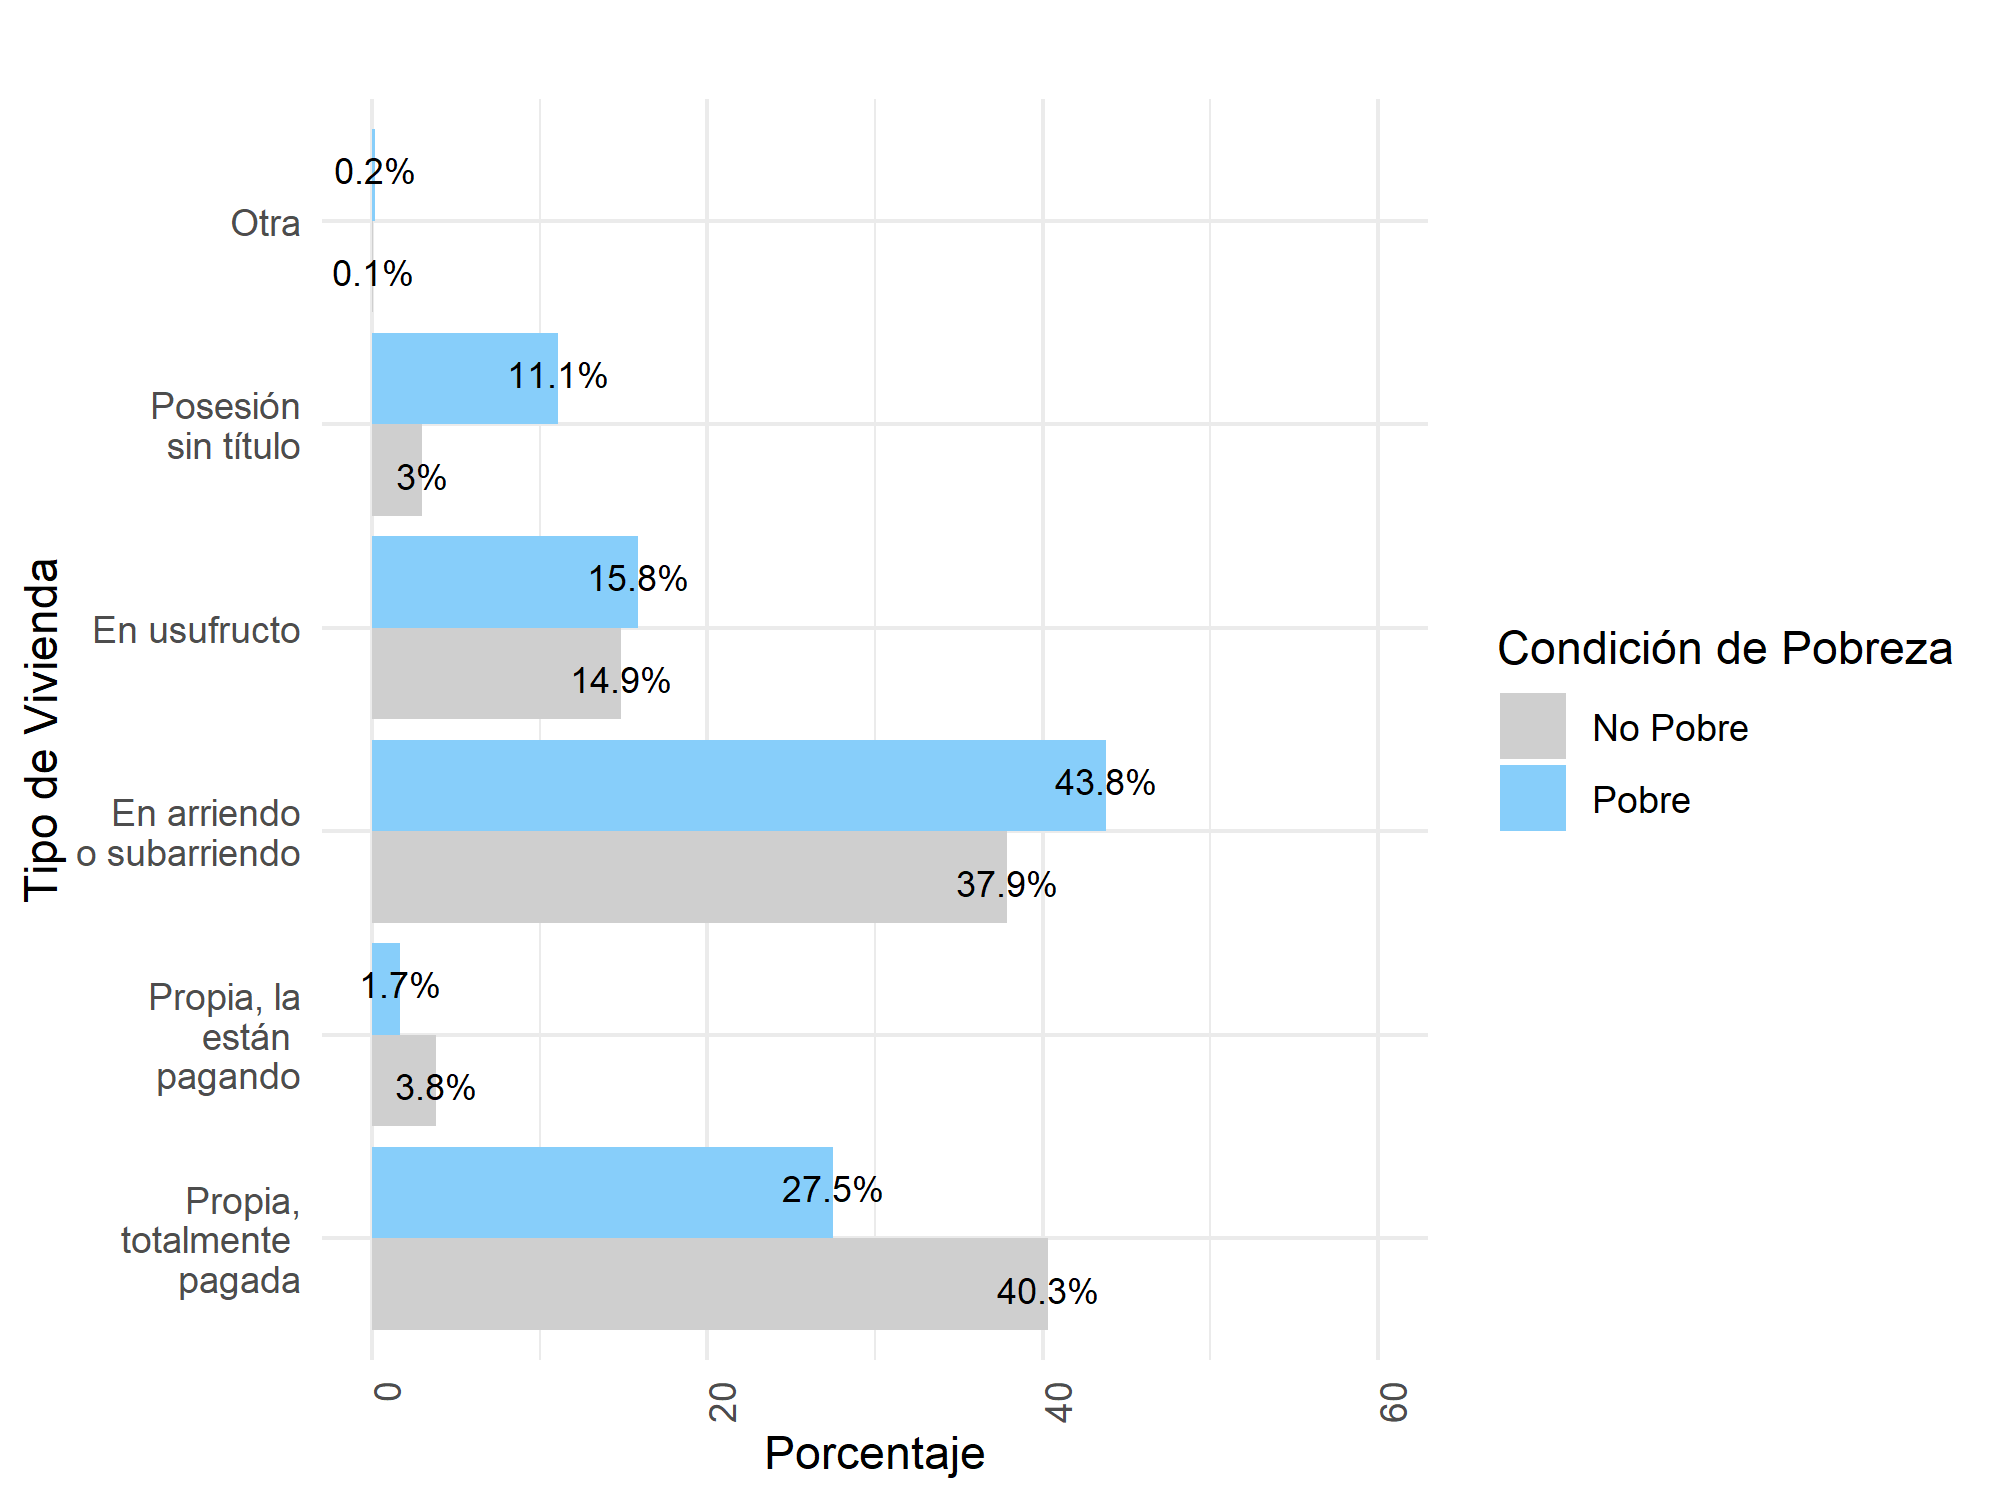
\includegraphics[width=0.6\linewidth]{Graficas/tipo_vivienda.png}
    \end{figure}


La Figura 2 muestra la distribución porcentual de la condición de pobreza en zonas rurales y urbanas. En las áreas rurales, el 14,1\% de la población es pobre, frente a un 8,2\% en las cabeceras urbanas. Esto indica que en estas zonas debería haber un enfoque mas agresivo de política que ayude a reducir la pobreza.\\

    \begin{figure}[H]
        \centering
            \caption{Condición de pobreza por zona}
        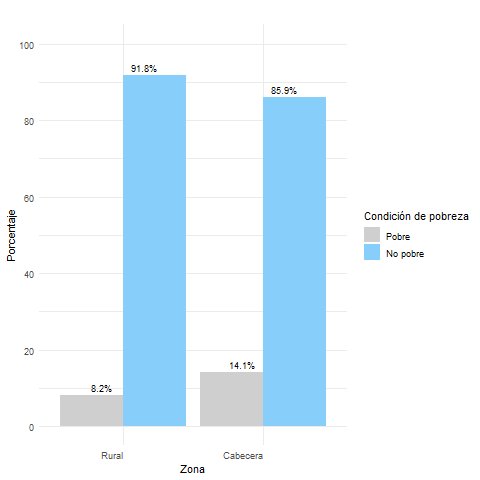
\includegraphics[width=0.5\linewidth]{Graficas/Clase.png}
    \end{figure}

  La Figura 3 muestra que existe una clara relación entre el nivel educativo alcanzado y la condición de pobreza. La mayoría de la población no pobre ha alcanzado el nivel universitario (54,4\%), mientras que solo el 28,1\% de las personas en situación de pobreza llega a este nivel. En cambio, los niveles de educación media, secundaria y primaria presentan mayores proporciones entre la población pobre, con un 38,5\%, 20,1\% y 12,8\%, respectivamente, frente a porcentajes menores en la población no pobre. Esto sugiere que un menor nivel educativo está asociado a una mayor prevalencia de pobreza, resaltando la importancia de la educación superior como un factor de reducción de la pobreza.
  
    \begin{figure}[H]
        \centering
            \caption{Máximo nivel educativo}
        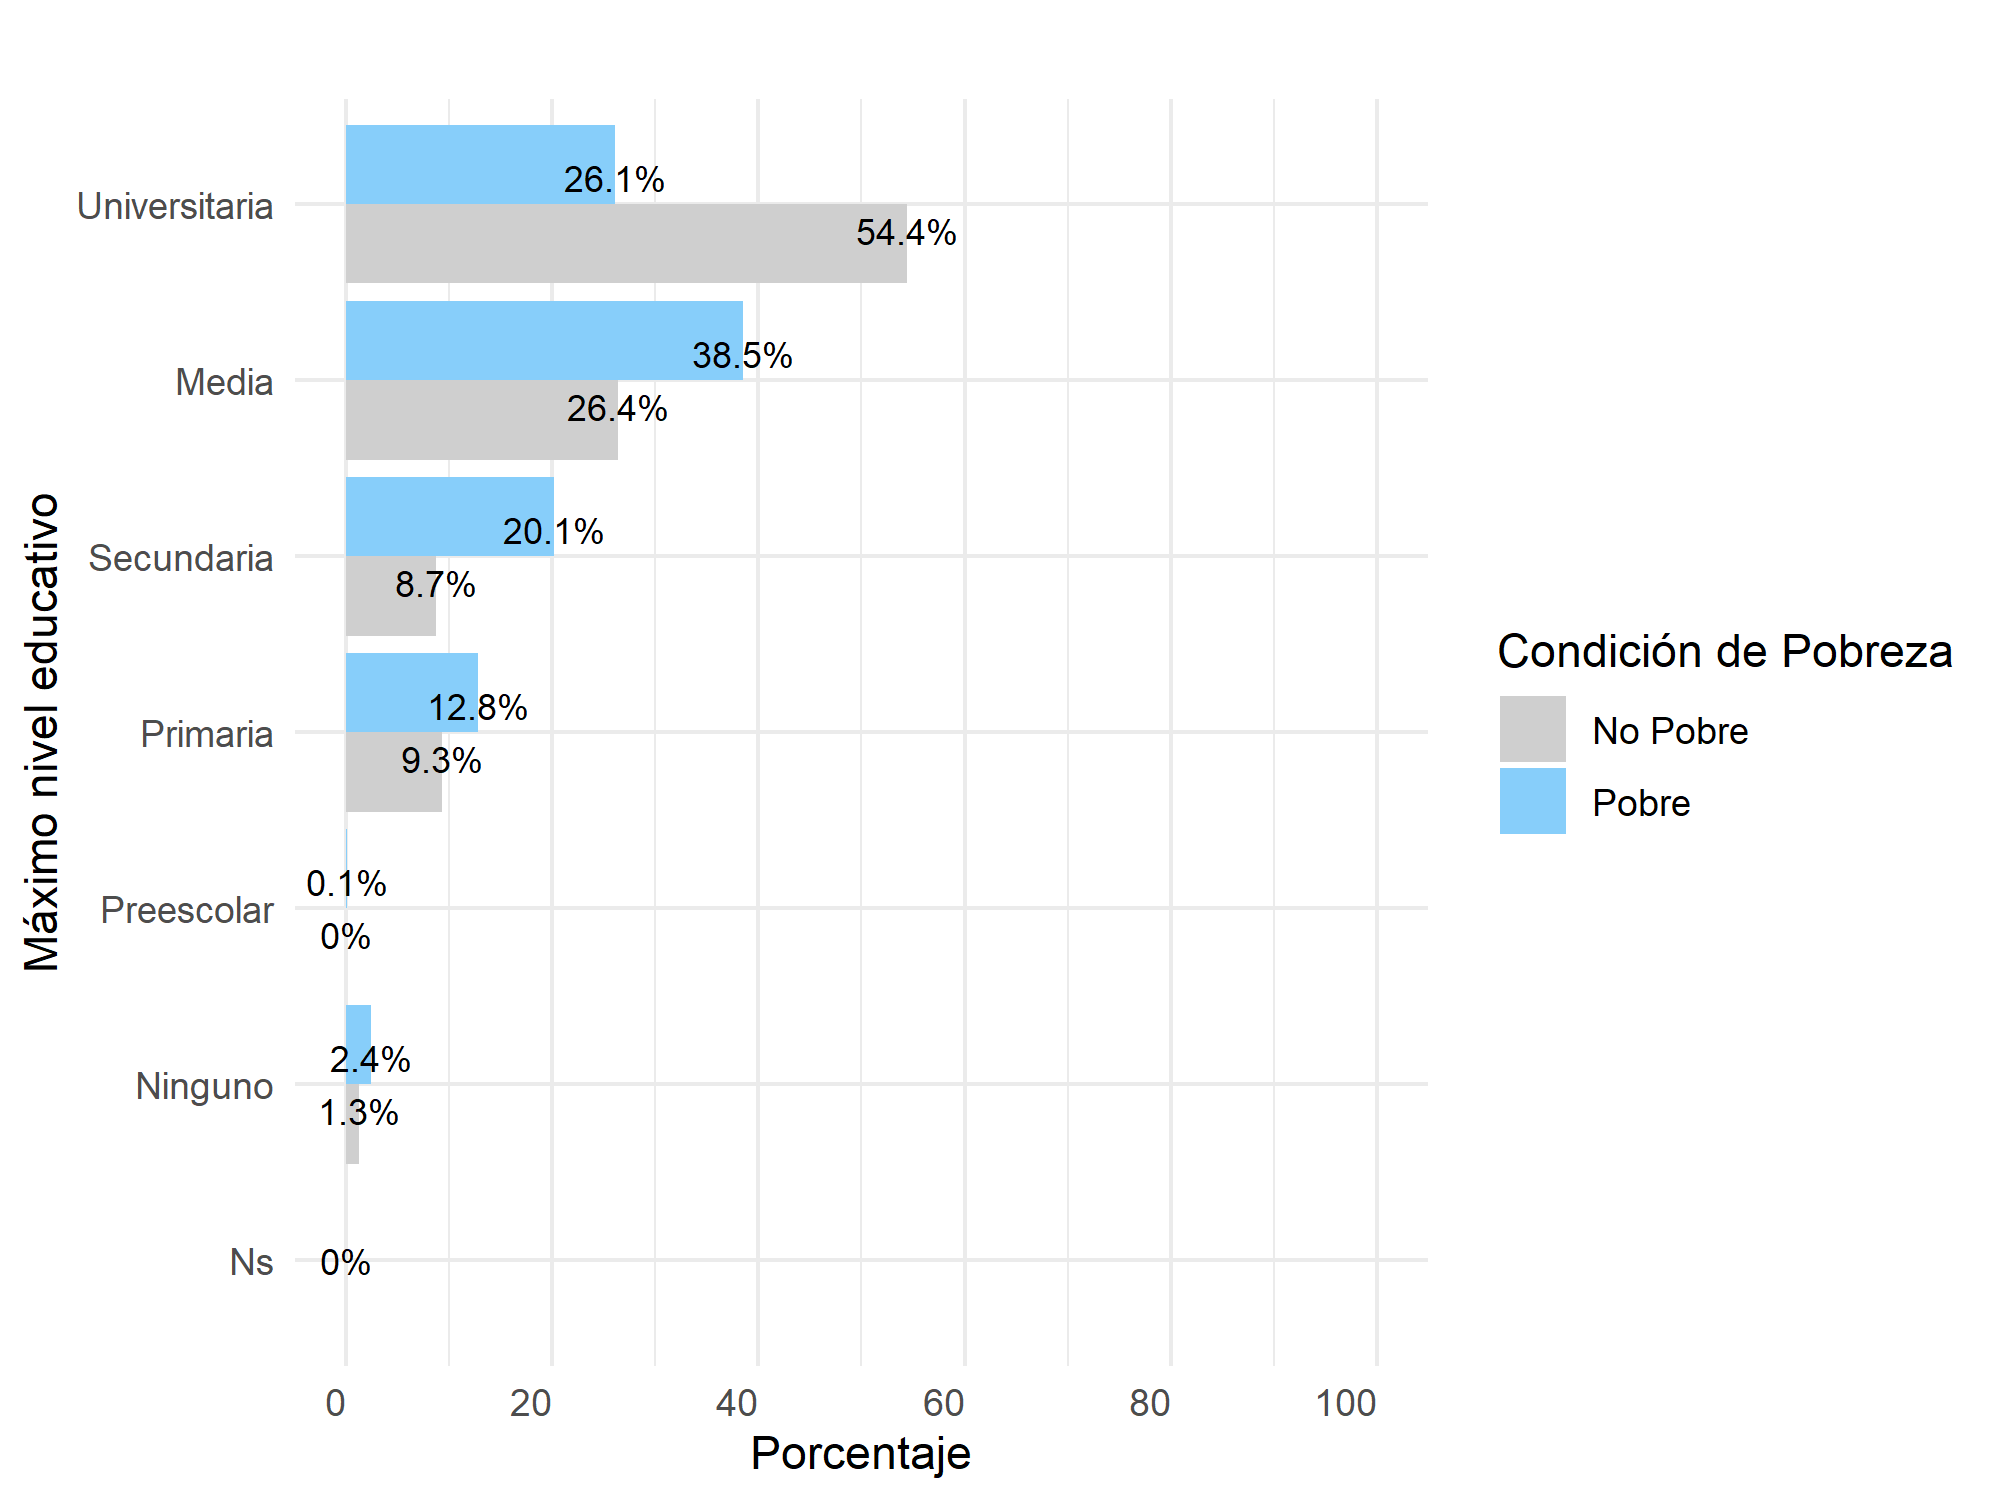
\includegraphics[width=0.6\linewidth]{Graficas/Educacion.png}
    \end{figure}

Al examinar la relación entre la situación de pobreza y el género de la jefatura del hogar, como se muestra en la Figura 4, se observa que los hogares encabezados por hombres presentan una menor incidencia de pobreza, con un 40,6\% de pobres frente al 46,8\% de las mujeres. Estos datos indican que los hogares con jefatura femenina enfrentan una mayor vulnerabilidad económica en comparación con los liderados por hombres, evidenciando una desigualdad en las condiciones económicas según el género de quien encabeza el hogar. Este hallazgo sugiere la necesidad de políticas focalizadas que aborden esta disparidad de género, promoviendo una mayor equidad económica y brindando apoyo específico a los hogares liderados por mujeres para reducir su vulnerabilidad ante la pobreza. \\


    \begin{figure}[H]
        \centering
            \caption{Género del jefe del hogar}
        
\includegraphics[width=0.5\linewidth]{Graficas/Jefatura.png}
    \end{figure}


Al comparar el número promedio de personas por hogar, se observa que los hogares clasificados como pobres tienen en promedio un mayor número frente a los no pobres (Figura 5). Esto puede estar asociado a una mayor carga económica y una posible limitación en el acceso a recursos y servicios básicos para todos los miembros del hogar. Al comparar el número de cuartos en la vivienda del hogar, se observa que los hogares pobres tienen en promedio menores cuartos (Figura 6). Esta diferencia sugiere que los hogares pobres, además de ser más grandes en términos de personas, cuentan con menos espacio, lo que podría estar asociado a condiciones de hacinamiento, con consecuencias adversas sobre la calidad de vida y el bienestar del hogar.\\

   \begin{figure}[H]
    \centering
    \begin{minipage}{0.5\textwidth}
        \centering
         \caption{Número de personas promedio}
        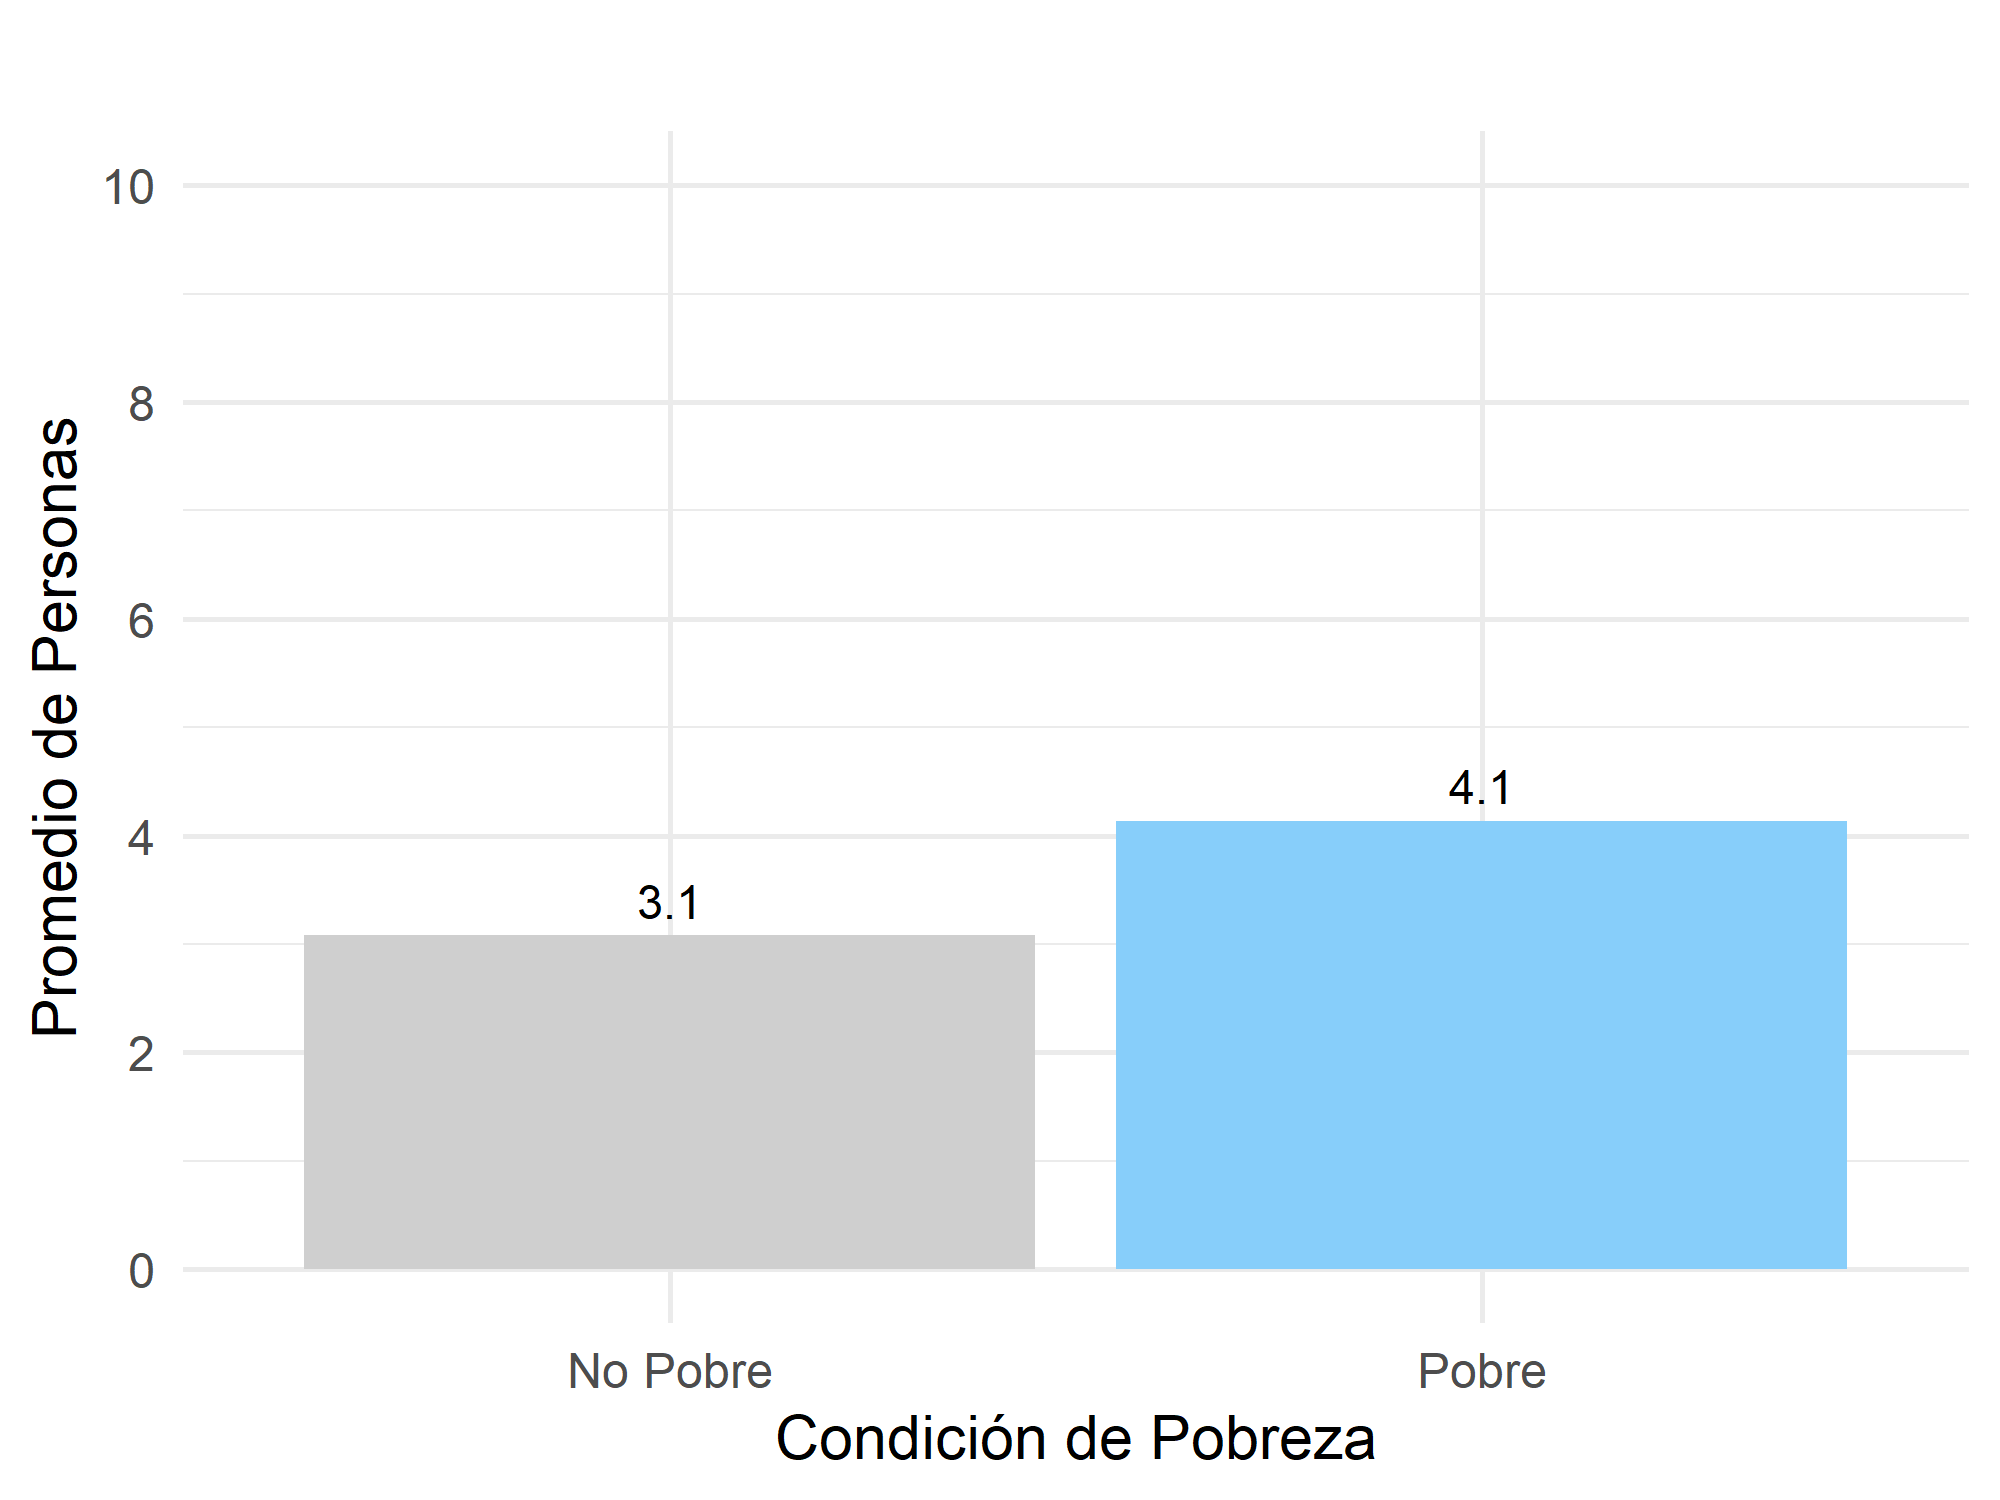
\includegraphics[width=\linewidth]{Graficas/personas_hogar.png}  
    \end{minipage}\hfill
    \begin{minipage}{0.5\textwidth}
        \centering
         \caption{Número de cuartos promedio}
        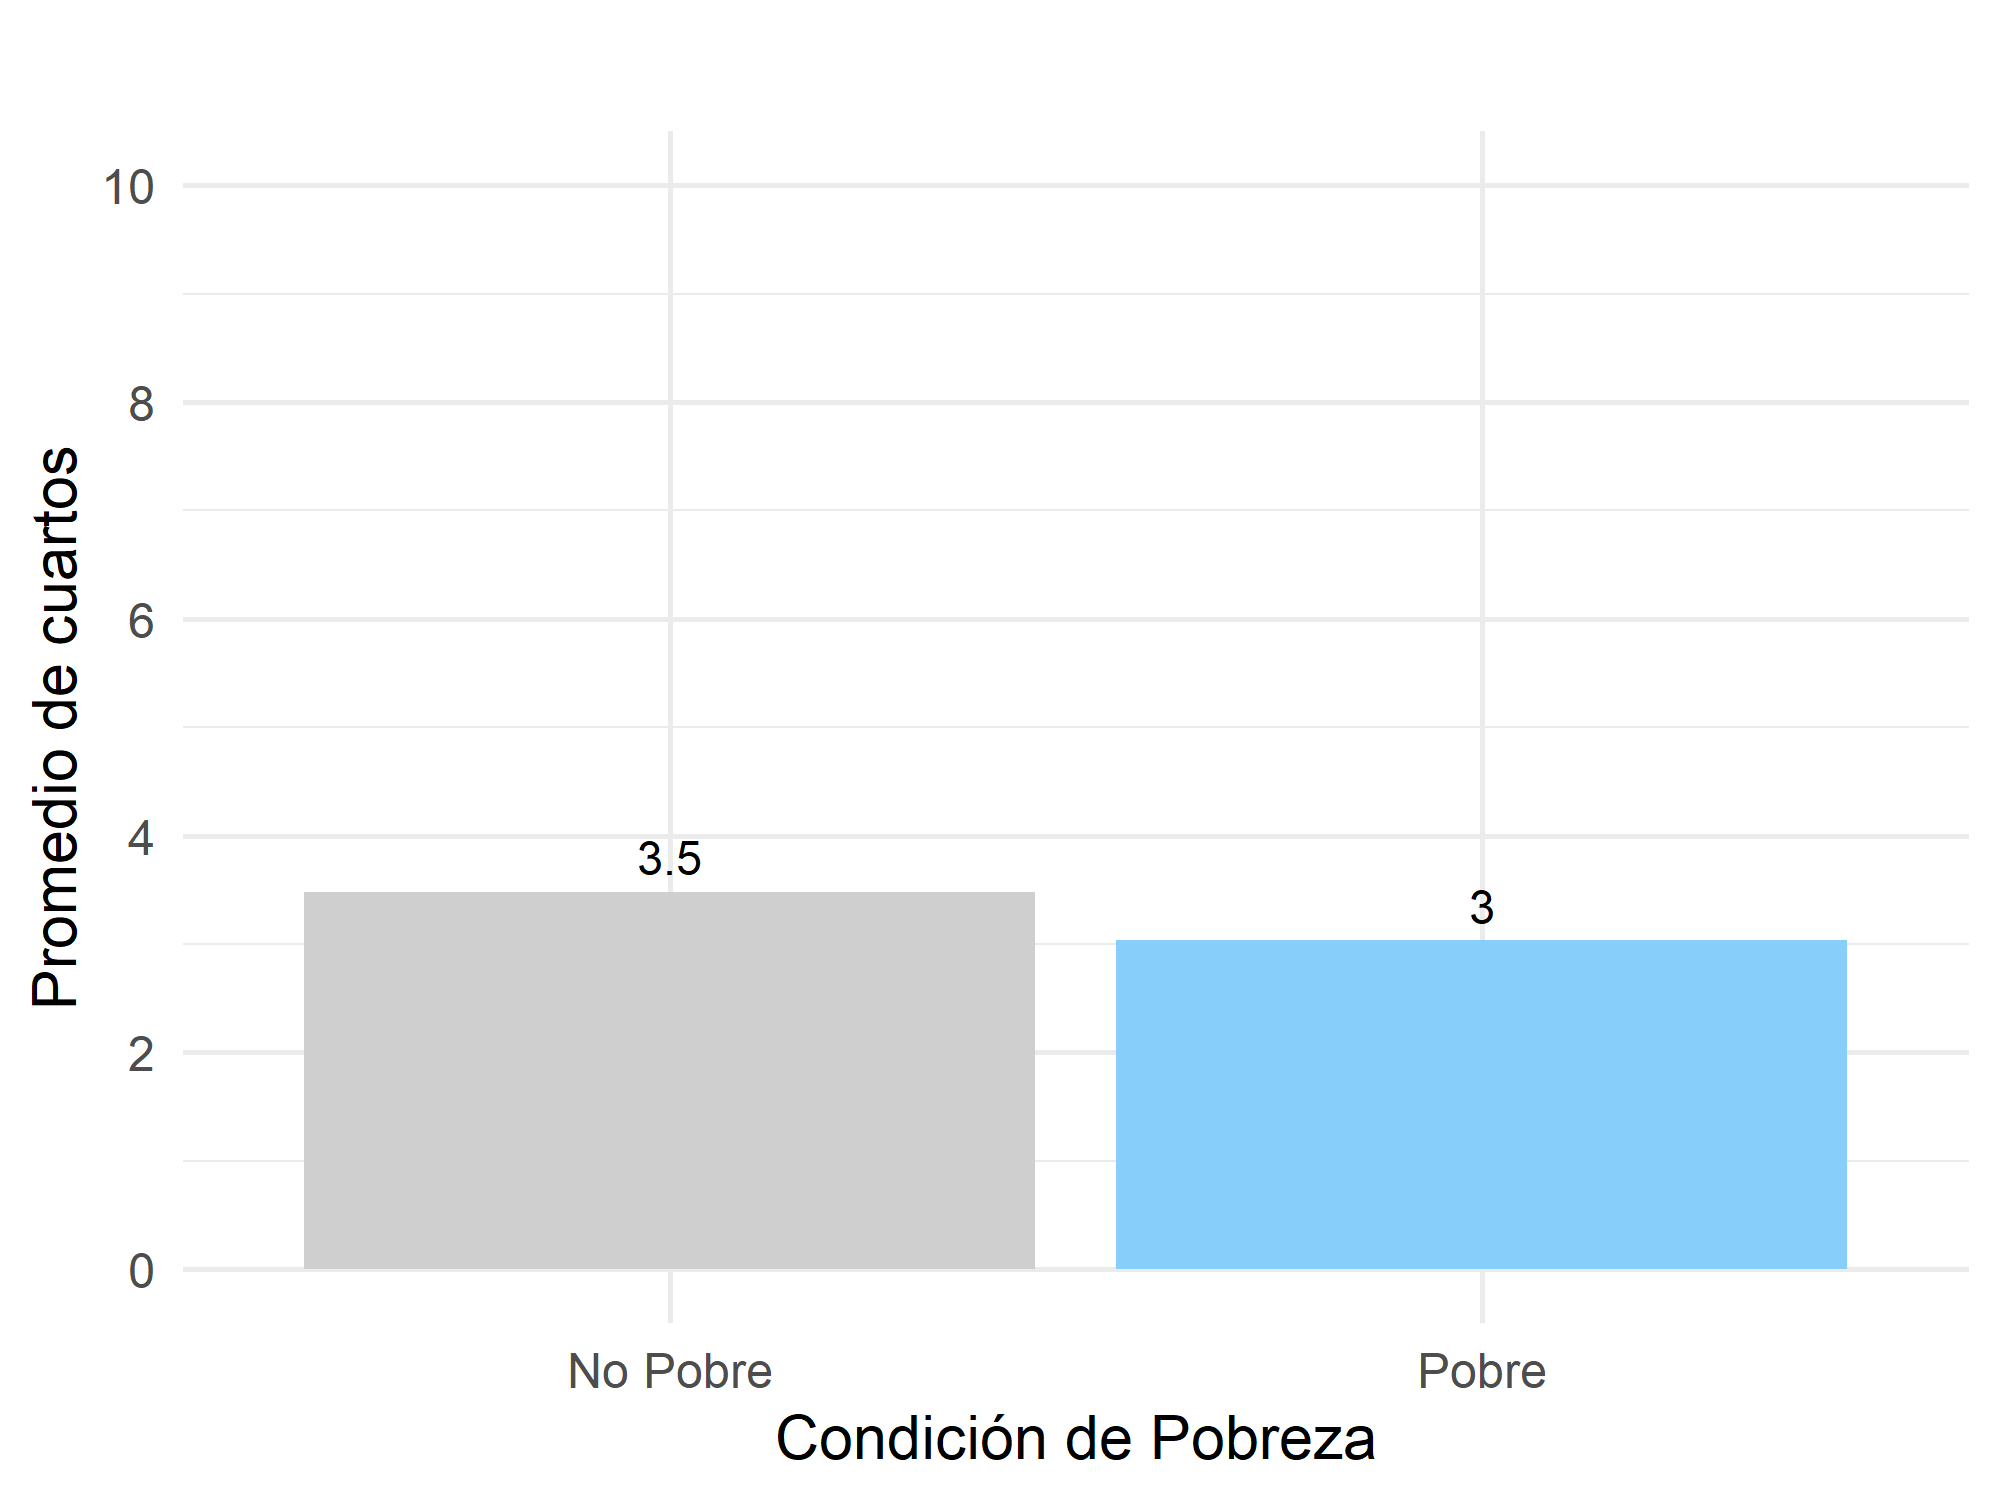
\includegraphics[width=\linewidth]{Graficas/num_cuartos.png} 
    \end{minipage}
\end{figure}

 Finalmente, las estadísticas de los datos utilizados en la base de datos original y la base de datos rebalanceada utilizada en el modelo final, se pueden consultar en los Anexos. A partir de la comparación entre la base de datos original y la rebalanceada mediante SMOTE, se observa que el número total de observaciones aumentó significativamente, pasando de 164.960 a 196.359, lo que es consecuencia directa del rebalanceo aplicado para mejorar la clasificación de la población pobre en Colombia. En ambos conjuntos de datos, tanto en la base original como en la base SMOTE usada en el modelo, variables clave para la clasificación de la población pobre en Colombia muestran comportamientos consistentes. Por ejemplo, la edad del jefe de hogar presenta una media de aproximadamente 49 años en la base original y 48,7 años en la base SMOTE, lo que indica que la mayoría de los jefes de hogar se encuentran en edades productivas.\\
 
 El número de personas por dormitorio es similar en ambos casos, con una media de alrededor de 1,7 y 1,87, lo que revela una tendencia moderada al hacinamiento, especialmente en los hogares más vulnerables, considerando que la media de cuartos donde duermen no alcanzan las dos unidades. Por otro lado, el número de mujeres por hogar tiene una media de alrededor de 1,74 y 1,86, lo que sugiere que en la mayoría de los hogares hay al menos una mujer, siendo un indicador importante en contextos donde la jefe del hogar es una mujer, lo cual podría relacionarse con mayores niveles de vulnerabilidad económica al ser históricamente aquellas que, aparte, son las principales encargadas de las tareas del hogar. El número de ocupados por hogar es aproximadamente 1,5 en ambas bases, lo que refleja que, en promedio, solo una persona en el hogar está ocupada, un indicador clave de las dificultades para generar ingresos suficientes cuando la muestra evidencia que al menos se encuentran 3 personas en el hogar. Además, el número total de subsidios por hogar presenta un valor medio cercano a 0.23, lo que indica que una proporción importante de los hogares accede a algún tipo de subsidio, pero este no representa un comportamiento generalizado.


\section{Modelos entrenados}

Como se mencionó anteriormente, la base de datos contaba con un desbalance donde solo el 20,01\% de los hogares son clasificados como pobres. Por ende se aplicó la técnica SMOTE (Synthetic Minority Over-sampling Technique) para generar observaciones sintéticas de la clase minoritaria. Dicho esto, se aplicó sobre esta base y sobre la base original diferentes técnicas de clasificación que buscan lograr un mayor proceso de aprendizaje a partir de los datos y una predicción que llevara a un valor del F1 Score más cercano al 100\%. De esta manera, en cada modelo, de forma general, se separó la base de entrenamiento en un 85\% para el cálculo del modelo, algunos ajustado por la métrica F, y se realizó un testeo al interior de la muestra con el 15\% restante, antes de realizar la predicción con los datos de test por fuera de muestra en Kaggle.  A continuación se presentará los modelos utilizados en este ejercicio con una descripción breve del proceso de análisis. \\

En los análisis realizados se logran identificar por medio de la matriz de importancia de variables algunos predictores fundamentales de la base de entrenamiento para predecir la pobreza. Estas variables son buenos predictores porque reflejan aspectos clave de la situación económica de los hogares. El nivel educativo alcanzado maximo están directamente relacionados con mejores empleos e ingresos. El número de ocupados indica la capacidad de generación de ingresos, mientras que la afiliación a la seguridad social refleja estabilidad laboral y contratos de trabajo formales. Además, el número de menores de 6 años incrementa los gastos del hogar y reduce la capacidad laboral, lo que aumenta el riesgo de pobreza. Finalmente, los subsidios son indicadores de vulnerabilidad monetaria. 

\subsection{Regularización: Ridge y Elastic Net} \\

Para un acercamiento inicial del problema de clasificación de pobreza se realizó un acercamiento mediante penalización por Elastic Net. En primer lugar, se entrenó un modelo utilizando diferentes tipos de indicadores de pobreza. Comúnmente, basados en los indicadores de pobreza multidimensional utilizados en la práctica, se tomaron variables referentes al hogar, tales como hacinamiento, pago de arriendo y total de ocupados y desempleados, así como variables indirectas como menores de edad con trabajo y características del jefe del hogar como la condición de que este sea una mujer.\\

De este ejercicio se probaron diferentes niveles de penalización, en los cuales se encontró el valor óptimo del parámetro Lambda  y Alpha. De estas pruebas se logró identificar que un mayor nivel de regularización fue beneficioso para la clasificación fuera de muestra, en la que, de los diferentes modelos planteados, se mantuvo un mismo valor de Lambda igual al 0,001 y un valor de Alpha igual a 1. \\

Adicionalmente se empleo el modelo de regularizacion Ridge con variables como tipo de vivienda, número de cuartos, educación y edad del jefe del hogar, entre otras. A través de validación cruzada de 10 pliegues, se determinó un lambda óptimo de 0.0138. El modelo alcanzó una precisión del 84.1\% y un F1-Score de 0.48, lo que indica un rendimiento aceptable, aunque con margen de mejora en la detección de los casos de pobreza (recall del 37\%). En este caso se utilizo la base original de entrenamiento sin remuestreo SMOTE.

\subsection{Logit}

Se realizó un análisis por medio del modelo Logit para observar la capacidad de aprendizaje. A partir de los resultados anteriores se procedió a probar diferentes combinaciones de las variables características de los hogares y de las condiciones del jefe del hogar. Tomando en cuenta el resultado del F1-Score se encontró que la inclusión de variables como Cabecera y la edad del jefe del hogar beneficio la clasificación de la pobreza dentro de la muestra, dando como resultado un aumento del score en Kaggle. De esta forma, también se incluyo en el modelo un proceso de validación cruzada con un total de 10 particiones y se incluyo un proceso de estandarización y centrado para considerar los casos en las que la escala de la variable dificulta su cálculo. Logrando un puntaje F1 de 0.558.

\subsection{Linear Discriminant Analysis}

El modelo de Análisis Discriminante Lineal (LDA) para el problema de clasificación se entrenó usando un conjunto de variables como el tipo de vivienda, ubicación, nivel educativo, características del jefe del hogar, entre otras. Este modelo puede ser ideal dado el desbalance de las muestras, es por eso que el entrenamiento de este modelo se realizó bajo la base original de entrenamiento y no sobre la base rebalanceada con SMOTE.  \\

El proceso de entrenamiento incluyó una validación cruzada de 10 veces, lo que permitió medir la robustez del modelo frente a diferentes particiones de los datos. La precisión (accuracy) del modelo fue de 83,96\%, lo que significa que el modelo predijo correctamente en un alto porcentaje de los casos. Sin embargo, dado el desbalance en las clases, se presta especial atención al F1-Score, que fue de 0.520 para la clase positiva ("pobre"), con un recall de 0,413.




\subsection{Random Forest}

El modelo utilizado de \textit{Random Forest} fue entrenado con 62 variables predictoras utilizando validación cruzada con 5 particiones. Entre los hiperparámetros clave, se estableció que se consideran 20 variables en cada división de los nodos, y un mínimo de 20 observaciones por nodo terminal. El modelo utiliza el índice de Gini como criterio de división y fue entrenado con 100 árboles. \\

El rendimiento del modelo en el conjunto de entrenamiento es sólido, con una precisión del 91,04\%, un Kappa de 0.8158, y un AUC de 0.8406. El \textit{F1-Score} en entrenamiento es 0.9233, lo que indica un buen equilibrio entre precisión y \textit{recall}. Sin embargo, en el conjunto de prueba, el \textit{F1-Score} cae a 0.65, lo que sugiere que el modelo podría estar algo sobreajustado y beneficiarse de ajustes adicionales para mejorar su generalización en datos nuevos.


\subsection{Quadratic Discriminant Analysis}

El modelo de Análisis Discriminante Cuadrático (QDA). Entre las variables incluidas en el modelo se encuentran el tipo de vivienda, el número de cuartos, la ubicación en cabecera, el nivel educativo del jefe de hogar, y otras relacionadas con ocupación y subsidios. \\

El modelo QDA fue entrenado con 140,217 muestras y validado mediante una validación cruzada de 10 particiones. Obtuvo un valor Kappa de 0.38, lo que indica un rendimiento moderado, especialmente dada la proporción desbalanceada de hogares pobres utilizada en este caso también el conjunto de datos (solo el 20\%). El F1-Score fue 0.501, reflejando un equilibrio entre precisión y recall, aunque el recall para identificar hogares pobres fue limitado con un valor de 0.494. En este caso se uso la base de entrenamiento sin el remuestreo.


\subsection{K-Nearest Neighbours}

Este modelo clasifica una observacion basado en los K vecinos mas cercanos. Es sensible a la escala de los datos y sufre en alta dimensionalidad debido a la pérdida de significado de las distancias. Se ajusto el valor de k (vecinos) entre 13 y 50. Tras seleccionar el k óptimo, el cual fue 28, se aplicó el modelo tanto a datos de prueba internos como externos. El F1-Score de 0.42552 refleja un bajo equilibrio entre precisión y recall en el modelo, lo que indica que el KNN tiene dificultades para identificar correctamente los hogares pobres. A pesar de una precisión decente de 67.97\%, el recall es bajo (30.97\%), lo que significa que el modelo deja de identificar muchos hogares pobres, afectando su rendimiento general en términos de predicción de pobreza. En este caso tambien se utilizo la base de entrenamiento sin remuestreo.




\section{Resultados}

A continuación, se presenta una comparación de los resultados de todos los modelos utilizados en el proceso de predicción de la pobreza de los hogares que fueron descritos en la sección anterior, utilizando la información de la base de datos de entrenamiento rebalanceada. Específicamente, la Tabla \ref{tab:modelos} muestra una comparación del desempeño dentro de la muestra de entrenamiento y fuera de muestra de acuerdo con la puntuación de Kaggle.\\

\vspace{-0.5cm}
\begin{table}[h!]
\centering
\caption{Comparación del desempeño de los modelos en la predicción de la pobreza}
\label{tab:modelos}
\begin{tabular}{|c|l|c|c|}
\hline
\textbf{Modelo} & \textbf{Algoritmo} & \textbf{F1 – Train} & \textbf{F1 – Test (Kaggle)} \\ \hline
1              & Logit & 0,550  & 0,558 \\ \hline
2              & Linear Discriminant Analysis (LDA) & 0.508 & 0,520 \\ \hline
3              & Elastic Net & 0,707 & 0,544 \\ \hline
4              & k vecinos más próximos & 0,425 & 0,432 \\ \hline
5              & Árbol de clasificación & 0,526 & 0,568 \\ \hline
6              & Random Forest & 0,953 & 0,655 \\ \hline
7              & XGBoost & 0,906 & 0,683 \\ \hline
9              & Ridge & 0,482 & 0,491 \\ \hline

\end{tabular}

\scriptsize{\textbf{Nota:} En esta tabla se presenta solamente el mejor resultado de cada uno de los algoritmos empleados. Por ejemplo, si en Kaggle se subieron 3 predicciones de un algoritmo, se muestran los resultados solo del modelo con mejor predicción.
} \\

\normalsize
\end{table}

De todos los modelos analizados, el mejor resultado fuera de muestra se obtuvo empleando el algoritmo XGBoost, donde la métrica F1 alcanzó un valor de 0.683 en Kaggle. Este algoritmo representó una mejora importante comparativamente a la segunda mejor predicción obtenida a través de Random Forest. Para ello se utilizaron todas las variables descritas en la sección anterior y disponibles en el anexo, sobre la base de datos rebalanceada y, a través de un proceso de validación cruzada, se obtuvieron los hiperparámetros que maximizaron dicha métrica (Tabla \ref{tab:hiperparametros}).\\

La combinación del total de hiperparámetros evaluados derivó en una estimación de un total de 972 modelos. A pesar de que es un número alto de modelos, con el objetivo de limitar el costo computacional, se restringió este universo de combinaciones al establecer valores máximos en ciertos hiperparámetros de acuerdo con los resultados obtenidos en análisis anteriores. En particular, se evaluó previamente a través del algoritmo de Random Forest la posibilidad de incluir entre 500, 750 y 1000 árboles, y se encontró un mejor resultado para 500. Dado esto, el número máximo de árboles se limitó a 500. Asimismo, se concluyó que el valor máximo de observaciones mínimas por hoja debía ser 30, ya que valores mayores como 50 y 100 no mejoraron los resultados.\\

\begin{table}[h!]
\centering
\caption{Hiperparámetros evaluados y seleccionados para XGBoost}
\label{tab:hiperparametros}
\begin{tabular}{|l|c|c|}
\hline
\textbf{Parámetros} & \textbf{Evaluados} & \textbf{Seleccionado} \\ \hline
Número de árboles (nrounds) & 100; 300; 500 & 500 \\ \hline
Profundidad máxima (max\_depth) & 2; 4; 6 & 6 \\ \hline
Tasa de aprendizaje (eta) & 0.01; 0.05; 0.1 & 0.05 \\ \hline
Observaciones mínimas por hoja (min\_child\_weight) & 10; 20; 30 & 20 \\ \hline
Parámetro de regularización (gamma) & 0; 0.5; 1 & 0 \\ \hline
Proporción de predictores (colsample\_bytree) & 0.33; 0.66 & 0.66 \\ \hline
Fracción de datos (subsample) & 0.4; 0.8 & 0.8 \\ \hline
\end{tabular}
\vspace{0.5mm}

\scriptsize
\textbf{Nota:} Entre paréntesis se muestra la identificación del hiperparámetro en el lenguaje de programación de R.
\end{table}

\vspace{0.5cm}

En total, se usaron 63 regresores, cuya importancia relativa se presenta en la Tabla 5 del anexo. La variable más importante en el proceso de clasificación fue el régimen de seguridad social subsidiado de la persona cabeza de hogar. La segunda variable más importante fue el total de personas en el hogar afiliadas al régimen de salud subsidiado. Este resultado sugiere que el régimen de seguridad social es un buen predictor de la pobreza en Colombia, indicando que este tipo de subsidios puede estar correctamente focalizado hacia los hogares pobres. La tercera variable más relevante es el número de ocupados en el hogar, lo que es coherente desde un punto de vista económico, ya que menos personas ocupadas en un hogar pueden llevar a ingresos conjuntos más bajos, lo que puede derivar en una mayor probabilidad de que el hogar sea pobre. Sin embargo, se reconoce que esta relación no es estricta, ya que puede haber casos en los que una sola persona con altos ingresos sostenga a la familia o que se trate de un hogar unipersonal.Finalmente, la cuarta variable más relevante fue una variable categórica que indica si la educación universitaria fue la máxima alcanzada en el hogar. Este resultado es consistente con la literatura económica, ya que el nivel educativo es un determinante del ingreso laboral, por lo que los hogares con al menos una persona con educación universitaria tienen menos probabilidad de ser pobres.


\section{Conclusiones}

Este estudio abordó la pregunta de cómo predecir con mayor precisión la pobreza en Colombia utilizando datos del DANE, aplicando diversas técnicas de Machine Learning. Entre los modelos entrenados, el que utilizó el algoritmo de XGBoost fue el que presentó el mejor rendimiento en términos predictivos, alcanzando un F1-Score de 0.683. Este resultado refleja la capacidad del modelo para equilibrar precisión y recall en la clasificación de los hogares según su condición de pobreza, a pesar del desbalance en los datos, donde solo el 20\% de los hogares se clasificaron como pobres. \\

La precisión del modelo XGBoost en este contexto puede explicarse por su capacidad de manejar grandes volúmenes de datos y captar relaciones complejas entre variables. Las variables más influyentes en el modelo incluyeron el acceso a la seguridad social, el número de ocupados y el nivel educativo del jefe de hogar. Estas variables reflejan los factores socioeconómicos clave que pueden determinar o predicen consistentemente la pobreza. \\

Para mejorar los resultados futuros, se recomienda seguir explorando técnicas adicionales para manejar el desbalance en los datos, como el aprendizaje con costos sensibles, así como incorporar más variables relacionadas con la salud y el acceso a servicios. En conclusión, XGBoost demostró ser una herramienta eficaz para identificar hogares vulnerables, y puede servir como base para diseñar políticas sociales más precisas y menos costosas para combatir la pobreza en Colombia.

\section{Referencias}

\begin{itemize}
    \item A. B. Atkinson (1987). On the Measurement of Poverty.
    \item Banco Mundial. (2023). Poverty and Shared Prosperity 2023. Banco Mundial.
    \item Departamento Administrativo Nacional de Estadística (DANE). (2023).Pobreza Monetaria en Colombia. DANE.
    \item Sosa, W., \& Cornejo, M. (2022). Predicciones agregadas de pobreza con información a escala micro y macro: Evaluación, diagnóstico y propuestas. CEPAL.
    \item Muñetón-Santa, G., & Manrique-Ruiz, L. C. (2023). Predicting multidimensional poverty with machine learning algorithms: an open data source approach using spatial data. Social Sciences, 12(5), 296.
    \item Sabogal, H., García-Bedoya, O., & Granados, O. (2021). Un análisis de la pobreza en Colombia basado en aprendizaje automático.


\end{itemize}





\section{Anexos}

\subsection{Ecuación de modelo LDA}

\begin{equation}
\begin{aligned}

$Pobre_i = \beta_0 + \beta_1 tipo\_vivienda_i + \beta_2 Cabecera_i + \beta_3 Nper_i + \beta_4 Dominio_i + \beta_5 Departamento_i + \beta_6 n\_cuartos_i + \beta_7 maxEducLevel_i + \beta_8 Head\_Ocupacion_i + \beta_9 Head\_Mujer_i + \beta_{10} rsubsidiado_i + \beta_{11} nsubsidios_i + \beta_{12} Head\_EducLevel_i + \beta_{13} Head\_Cot\_pension_i + \beta_{14} Head\_ocupado_i + \beta_{15} Head\_edad_i + \beta_{16} Head\_Afiliado\_SS_i + \beta_{17} nmenores\_6_i + \beta_{18} nincapacitados_i + \epsilon_i$


\end{aligned}
\end{equation}


\subsection{Ecuación de modelo QDA}

\begin{equation}
\begin{aligned}

$Pobre_i = \beta_0 + \beta_1 tipo\_vivienda_i + \beta_2 Cabecera_i + \beta_3 Nper_i + \beta_4 n\_cuartos_i + \beta_5 nmenores\_6_i + \beta_6 Head\_Mujer_i + \beta_7 rsubsidiado_i + \beta_8 nsubsidios_i + \beta_9 Head\_EducLevel_i + \beta_{10} Head\_Cot\_pension_i + \beta_{11} Head\_ocupado_i + \beta_{12} Head\_edad_i + \beta_{13} Head\_Afiliado\_SS_i + \beta_{14} nocupados_i + \beta_{15} nincapacitados_i + \epsilon_i$


\end{aligned}
\end{equation}

\subsection{Ecuación de modelo Ridge}

\begin{equation}
\begin{aligned}
\hat{y}_i = & \beta_0 + \beta_1 \cdot \text{x}_{\text{tipo\_vivienda}, i} + \beta_2 \cdot \text{x}_{\text{Cabecera}, i} + \beta_3 \cdot \text{x}_{\text{Nper}, i} \\
& + \beta_4 \cdot \text{x}_{\text{Dominio}, i} + \beta_5 \cdot \text{x}_{\text{Departamento}, i} + \beta_6 \cdot \text{x}_{\text{n\_cuartos}, i} \\
& + \beta_7 \cdot \text{x}_{\text{maxEducLevel}, i} + \beta_8 \cdot \text{x}_{\text{Head\_Ocupacion}, i} + \beta_9 \cdot \text{x}_{\text{Head\_Mujer}, i} \\
& + \beta_{10} \cdot \text{x}_{\text{rsubsidiado}, i} + \beta_{11} \cdot \text{x}_{\text{nsubsidios}, i} + \beta_{12} \cdot \text{x}_{\text{Head\_EducLevel}, i} \\
& + \beta_{13} \cdot \text{x}_{\text{Head\_Cot\_pension}, i} + \beta_{14} \cdot \text{x}_{\text{Head\_ocupado}, i} + \beta_{15} \cdot \text{x}_{\text{Head\_edad}, i} \\
& + \beta_{16} \cdot \text{x}_{\text{Head\_Afiliado\_SS}, i} + \beta_{17} \cdot \text{x}_{\text{nmenores\_6}, i} + \beta_{18} \cdot \text{x}_{\text{nincapacitados}, i} \\
& + \lambda \sum_{j=1}^{18} \beta_j^2
\end{aligned}
\end{equation}

\subsection{Ecuación de modelo Logit}


\begin{equation}
\begin{aligned}
\hat{y}_i = & \frac{1}{1 + e^{-\left( \beta_0 + \beta_1 \cdot maxEducLevel_i + \beta_2 \cdot Dominio_i + \beta_3 \cdot n\_cuartos_i + \beta_4 \cdot Nper_i \right.}} \\
& \left. + \beta_5 \cdot nocupados_i + \beta_6 \cdot Cabecera_i + \beta_7 \cdot Head\_Ocupacion_i + \beta_8 \cdot Head\_edad_i \right)
\end{aligned}
\end{equation}

\subsection{Ecuación de modelo Elastic-Net}

\begin{equation}
\begin{aligned}
\hat{y}_i = & \beta_0 + \beta_1 \cdot hacinamiento_i + \beta_2 \cdot nocupados_i + \beta_3 \cdot ndesempleados_i + \beta_4 \cdot ntrabajo\_menores_i \\
& + \beta_5 \cdot Head\_Mujer_i + \beta_6 \cdot Pago\_Arriendo_i + \beta_7 \cdot n\_cuartos\_duermen_i + \beta_8 \cdot n\_cuartos_i \\
& + \beta_9 \cdot Head\_ocupado_i + \beta_{10} \cdot Head\_Afiliado\_SS_i + \beta_{11} \cdot Head\_Cot\_pension_i \\
& + \lambda \sum_{j=1}^{11} \left( \alpha \cdot |\beta_j| + (1 - \alpha) \cdot \beta_j^2 \right)
\end{aligned}
\end{equation}





\subsection{Tabla de estadísticas de las variables en el modelo final}


% Table created by stargazer v.5.2.3 by Marek Hlavac, Social Policy Institute. E-mail: marek.hlavac at gmail.com
% Date and time: dom, oct. 20, 2024 - 3:04:14 p. m.
\begin{table}[!htbp] \centering 
  \caption{Estadísticas básicas de las variables en la base original} 
  \label{} 
  \resizebox{\textwidth}{!}{ % Ajusta el tamaño de la tabla al ancho del texto
  \begin{tabular}{@{\extracolsep{5pt}}lccccc} 
  \\[-1.8ex]\hline 
  \hline \\[-1.8ex] 
  Statistic & \multicolumn{1}{c}{N} & \multicolumn{1}{c}{Mean} & \multicolumn{1}{c}{St. Dev.} & \multicolumn{1}{c}{Min} & \multicolumn{1}{c}{Max} \\ 
  \hline \\[-1.8ex] 
  Clase del hogar & 164,960 & 1.094 & 0.292 & 1 & 2 \\ 
  Número de cuartos & 164,960 & 3.390 & 1.239 & 1 & 98 \\ 
  Número de cuartos donde se duerme & 164,960 & 1.989 & 0.898 & 1 & 15 \\ 
  Número de personas en el hogar & 164,960 & 3.292 & 1.775 & 1 & 28 \\ 
  Número de personas en la unidad de gasto & 164,960 & 3.280 & 1.772 & 1 & 28 \\ 
  Personas por dormitorio & 164,960 & 1.728 & 0.830 & 0.200 & 16.000 \\ 
  Número de mujeres & 164,960 & 1.740 & 1.180 & 0 & 14 \\ 
  Número de menores de 6 años & 164,960 & 0.333 & 0.626 & 0 & 9 \\ 
  Número de adultos & 164,960 & 0.467 & 0.721 & 0 & 6 \\ 
  Número de menores trabajando & 164,960 & 0.024 & 0.169 & 0 & 5 \\ 
  Número de ocupados & 164,960 & 1.504 & 1.027 & 0 & 14 \\ 
  Número de desempleados & 164,960 & 0.182 & 0.446 & 0 & 6 \\ 
  Número de inactivos & 164,960 & 1.028 & 1.029 & 0 & 11 \\ 
  Número de personas en edad de trabajar & 164,960 & 2.714 & 1.400 & 0 & 19 \\ 
  Número de incapacitados & 164,960 & 0.043 & 0.219 & 0 & 4 \\ 
  Número de subsidios & 164,960 & 0.175 & 0.446 & 0 & 5 \\ 
  Régimen subsidiado & 164,960 & 1.202 & 1.484 & 0 & 14 \\ 
  Edad del jefe de hogar & 164,960 & 49.612 & 16.390 & 11 & 108 \\ 
  Pago de arriendo & 164,960 & 475,644.000 & 3,373,340.000 & 20 & 600,000,000 \\ 
  \hline \\[-1.8ex] 
  \end{tabular}
  }
\end{table} 

\scriptsize{\textbf{Nota:} En esta tabla 3 se presentan las principales estadísticas descriptivas de las variables numéricas del modelo de datos de entrenamiento original, resultado del proceso de limpieza y selección de variables.} \\




% Table created by stargazer v.5.2.3 by Marek Hlavac, Social Policy Institute. E-mail: marek.hlavac at gmail.com
% Date and time: dom, oct. 20, 2024 - 3:06:36 p. m.

\begin{table}[!htbp] \centering 
  \caption{Estadísticas básicas de las variables en la base modelo} 
  \label{} 
  \resizebox{\textwidth}{!}{ % Ajusta el tamaño de la tabla al ancho del texto
  \begin{tabular}{@{\extracolsep{5pt}}lccccc} 
  \\[-1.8ex]\hline 
  \hline \\[-1.8ex] 
  Statistic & \multicolumn{1}{c}{N} & \multicolumn{1}{c}{Mean} & \multicolumn{1}{c}{St. Dev.} & \multicolumn{1}{c}{Min} & \multicolumn{1}{c}{Max} \\ 
  \hline \\[-1.8ex] 
  Clase del hogar & 196,359 & 1.106 & 0.298 & 1.000 & 2.000 \\ 
  Número de cuartos & 196,359 & 3.282 & 1.184 & 1.000 & 98.000 \\ 
  Número de cuartos donde se duerme & 196,359 & 1.980 & 0.851 & 1.000 & 15.000 \\ 
  Número de personas en el hogar & 196,359 & 3.502 & 1.782 & 1.000 & 28.000 \\ 
  Número de personas en la unidad de gasto & 196,359 & 3.492 & 1.781 & 1.000 & 28.000 \\ 
  Personas por dormitorio & 196,359 & 1.870 & 0.899 & 0.200 & 15.000 \\ 
  Número de mujeres & 196,359 & 1.867 & 1.176 & 0.000 & 14.000 \\ 
  Número de menores de 6 años & 196,359 & 0.413 & 0.661 & 0.000 & 9.000 \\ 
  Número de adultos & 196,359 & 0.438 & 0.690 & 0.000 & 6.000 \\ 
  Número de menores trabajando & 196,359 & 0.029 & 0.175 & 0.000 & 5.000 \\ 
  Número de ocupados & 196,359 & 1.421 & 0.985 & 0.000 & 14.000 \\ 
  Número de desempleados & 196,359 & 0.219 & 0.460 & 0.000 & 6.000 \\ 
  Número de inactivos & 196,359 & 1.140 & 1.030 & 0.000 & 11.000 \\ 
  Número de personas en edad de trabajar & 196,359 & 2.781 & 1.373 & 0.000 & 19.000 \\ 
  Número de incapacitados & 196,359 & 0.048 & 0.218 & 0.000 & 4.000 \\ 
  Número de subsidios & 196,359 & 0.231 & 0.473 & 0.000 & 5.000 \\ 
  Régimen subsidiado & 196,359 & 1.503 & 1.541 & 0.000 & 14.000 \\ 
  Edad del jefe de hogar & 196,359 & 48.708 & 16.235 & 11.000 & 108.000 \\ 
  Pago de arriendo & 196,359 & 407,189.300 & 2,380,395.000 & 20.000 & 360,000,000.000 \\ 
  \hline \\[-1.8ex] 
  \end{tabular}
  }
\end{table} 
\scriptsize{\textbf{Nota:} En esta tabla 4 se presentan las principales estadísticas descriptivas de las variables numéricas del modelo de datos de entrenamiento rebalanceado mediante el proceso de SMOTE. Con base en los datos de la tabla original, el modelo crea variables sintéticas que permite un balance más adecuado de la variable a predecir y por ende es utilizado para la estimación del modelo final.}

\begin{table}[h!]
\centering
\caption{Importancia de variables en el modelo XGBoost}
\label{tab:importancia_variables}
\begin{tabular}{|l|c|}
\hline
\textbf{Variable}                   & \textbf{Overall} \\ \hline
Seguridad social subsidiada en Jefe del Hogar             & 0.209689         \\ \hline
Numero de personas afiliadas a seguridad social subsidiada                         & 0.143693         \\ \hline
Número de ocupados                           & 0.083005         \\ \hline
Maximo nivel de eduación del hogar: Universitario           & 0.059012         \\ \hline
Número de menores de seis años\_6                         & 0.055904         \\ \hline
Pago de arriendo                      & 0.048430         \\ \hline
Numero de personas inactivas en el hogar                           & 0.047788         \\ \hline
Numero de mujeres en el hogar                            & 0.034406         \\ \hline
Tipo de vivienda: Arrendada                     & 0.033706         \\ \hline
\end{tabular}
\end{table}


\begin{table}[!htbp] 
\centering 
\caption{Nombres de variables en la base de datos y su correspondiente interpretación}
\begin{tabular}{|l|l|}
\hline
\textbf{Variable Base de Datos} & \textbf{Nombre en Análisis} \\ 
\hline
Mujer & Mujer \\ 
Head & Jefe de Hogar \\ 
Head\_mujer & Jefe de Hogar Mujer \\ 
Head\_Educlevel & Nivel de educacion maximo\\ 
Head\_Ocupado & Jefe de Hogar Mujer \\ 
nmenores\_6 & Numero de menores de 6 Años \\ 
Adultos & Adultos \\ 
Trabajo\_menores & Trabajo de Menores \\ 
Incapacitado & Incapacitado \\ 
EducLevel & Nivel Educativo \\ 
exper\_ult\_trab & Experiencia Laboral \\ 
Afiliado\_SS & Afiliado a Seguridad Social \\ 
Reg\_subs\_salud & Régimen Subsidiado \\ 
Cot\_pension & Cotización a Pensión \\ 
Rec\_alimento & Recibe Alimentos \\ 
Rec\_vivienda & Recibe Vivienda \\ 
Rec\_otros & Otros Ingresos \\ 
Primas & Primas \\ 
Bonificaciones & Bonificaciones \\ 
Rec\_gub & Ayuda Gubernamental \\ 
Rec\_subsidio\_pais & Subsidio del País \\ 
Sub\_alim & Subsidio de Alimentación \\ 
Sub\_transp & Subsidio de Transporte \\ 
Sub\_famil & Subsidio Familiar \\ 
Sub\_educ & Subsidio de Educación \\ 
Uti\_transport & Uso de Transporte \\ 
Pago\_Arriendo & Pago de Arriendo \\ 
Valor\_Cuota & Valor Cuota \\ 
Hacinamiento & Hacinamiento \\ 
nincapacitados & Numero de incapacitados \\
n\_cuartos & Numero de cuartos \\
nsubsidios & Numero de subsidios \\
Nper & Numero de personas \\
\hline
\end{tabular} 
\end{table}









\end{document}
